\documentclass[../../main.tex]{subfiles}
\begin{document}
\section{Validity of the Reissner-Mindlin plate model}
In this section, the validity of a cantilever Reissner-Mindlin plate is investigates with reference to a three-dimensional plate model. In the previous section, it was shown that the beam models do not compare well when the parameter $b$ is ``too-large''. A plate model might be a better option.\\

Similarly to how the Timoshenko beam theory improves on the Euler-Bernoulli beam theory, the Reissner-Mindlin plate theory improves on classical plate theory by including the effect of shear stress. The Reisner-Mindlin plate theory is a two-dimensional theory. Therefore it is of interest to investigate the validity of such a plate model.Using \cite{LVV09} as a guide, the validity a cantilever Reisner-Mindlin plate model is investigated.\\

Figure \ref{fig:plate_sbs} shows the two cantilever plates side by side.
\FloatBarrier
\begin{figure}[h!]
	\scalebox{.8}{
		\makebox[\textwidth][c]{
			\caption{Side by side visualization of the cantilever plates.}
			\label{fig:plate_sbs}
			\centering
			\begin{minipage}[b]{0.8\linewidth}
				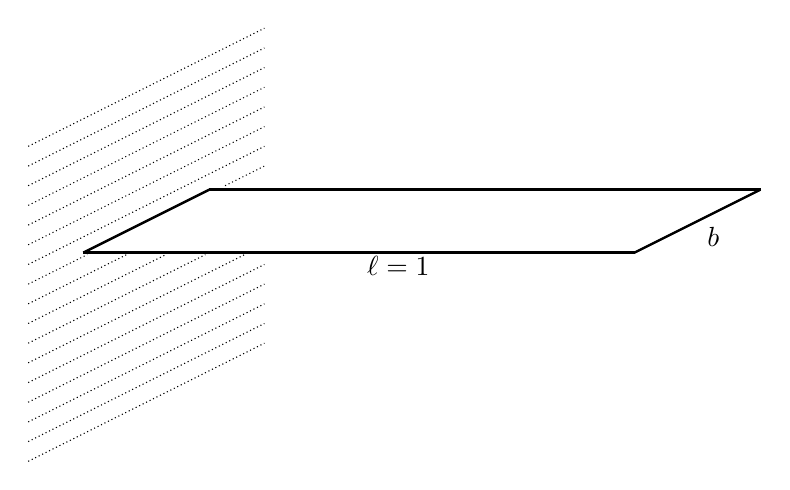
\begin{tikzpicture}
					\draw[line width = 0.3mm] (-0.8,-0.1) -- (6.2,-0.1);
					\draw[line width = 0.3mm] (0.8,0.7) -- (7.8,0.7);
					\draw[line width = 0.3mm] (-0.8,-0.1) -- (0.8,0.7);
					\draw[line width = 0.3mm] (6.2,-0.1) -- (7.8,0.7);
					
					
					
					\draw[scale=0.5, domain=-3:3, smooth, variable=\x,densely dotted] plot ({\x}, {0.5*\x+4});
					\draw[scale=0.5, domain=-3:3, smooth, variable=\x,densely dotted] plot ({\x}, {0.5*\x+3.5});
					\draw[scale=0.5, domain=-3:3, smooth, variable=\x,densely dotted] plot ({\x}, {0.5*\x+3});
					\draw[scale=0.5, domain=-3:3, smooth, variable=\x,densely dotted] plot ({\x}, {0.5*\x+2.5});
					\draw[scale=0.5, domain=-3:3, smooth, variable=\x,densely dotted] plot ({\x}, {0.5*\x+2});
					\draw[scale=0.5, domain=-3:3, smooth, variable=\x,densely dotted] plot ({\x}, {0.5*\x+1.5});
					\draw[scale=0.5, domain=-3:3, smooth, variable=\x,densely dotted] plot ({\x}, {0.5*\x+1});
					
					\draw[scale=0.5, domain=-3:-1.5, smooth, variable=\x,densely dotted] plot ({\x}, {0.5*\x+0.5});
					\draw[scale=0.5, domain=2:3, smooth, variable=\x,densely dotted] plot ({\x}, {0.5*\x+0.5});
					
					\draw[scale=0.5, domain=-3:-0.5, smooth, variable=\x,densely dotted] plot ({\x}, {0.5*\x});
					\draw[scale=0.5, domain=-3:0.5, smooth, variable=\x,densely dotted] plot ({\x}, {0.5*\x-0.5});
					\draw[scale=0.5, domain=-3:1.5, smooth, variable=\x,densely dotted] plot ({\x}, {0.5*\x-1});
					\draw[scale=0.5, domain=-3:2.5, smooth, variable=\x,densely dotted] plot ({\x}, {0.5*\x-1.5});
					\draw[scale=0.5, domain=-3:3, smooth, variable=\x,densely dotted] plot ({\x}, {0.5*\x-2});
					\draw[scale=0.5, domain=-3:3, smooth, variable=\x,densely dotted] plot ({\x}, {0.5*\x-2.5});
					\draw[scale=0.5, domain=-3:3, smooth, variable=\x,densely dotted] plot ({\x}, {0.5*\x-3});
					\draw[scale=0.5, domain=-3:3, smooth, variable=\x,densely dotted] plot ({\x}, {0.5*\x-3.5});
					\draw[scale=0.5, domain=-3:3, smooth, variable=\x,densely dotted] plot ({\x}, {0.5*\x-4});
					
					\node at (7.2,0.1) {$b$};
					\node at (3.2,-0.27) {$\ell = 1$};
										
					
					\draw[line width = 0.2mm] (0.8,0.7) -- (7.8,0.7);
					\draw[line width = 0.2mm] (-0.8,-0.1) -- (0.8,0.7);
					\draw[line width = 0.2mm] (6.2,-0.1) -- (7.8,0.7);
				\end{tikzpicture}
				\subcaption{Timoshenko Cantilever Beam}
			\end{minipage}
			\begin{minipage}[b]{0.8\linewidth}
				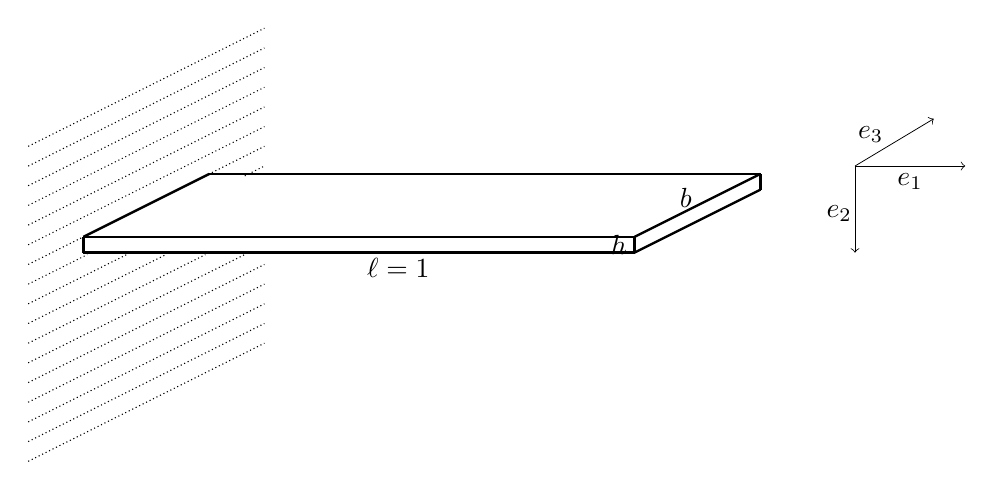
\begin{tikzpicture}
					\draw[line width = 0.3mm] (-0.8,0.1) -- (6.2,0.1);
					\draw[line width = 0.3mm] (-0.8,-0.1) -- (6.2,-0.1);
					\draw[line width = 0.3mm] (6.2,-0.1) -- (6.2,0.1);
					\draw[line width = 0.3mm] (-0.8,-0.1) -- (-0.8,0.1);
					
					\draw[line width = 0.3mm] (0.8,0.9) -- (7.8,0.9);
					\draw[line width = 0.3mm] (7.8,0.7) -- (7.8,0.9);
					
					\draw[line width = 0.3mm] (-0.8,0.1) -- (0.8,0.9);
					\draw[line width = 0.3mm] (6.2,0.1) -- (7.8,0.9);
					\draw[line width = 0.3mm] (6.2,-0.1) -- (7.8,0.7);
					
					
					
					\draw[scale=0.5, domain=-3:3, smooth, variable=\x,densely dotted] plot ({\x}, {0.5*\x+4});
					\draw[scale=0.5, domain=-3:3, smooth, variable=\x,densely dotted] plot ({\x}, {0.5*\x+3.5});
					\draw[scale=0.5, domain=-3:3, smooth, variable=\x,densely dotted] plot ({\x}, {0.5*\x+3});
					\draw[scale=0.5, domain=-3:3, smooth, variable=\x,densely dotted] plot ({\x}, {0.5*\x+2.5});
					\draw[scale=0.5, domain=-3:3, smooth, variable=\x,densely dotted] plot ({\x}, {0.5*\x+2});
					\draw[scale=0.5, domain=-3:3, smooth, variable=\x,densely dotted] plot ({\x}, {0.5*\x+1.5});
					\draw[scale=0.5, domain=-3:3, smooth, variable=\x,densely dotted] plot ({\x}, {0.5*\x+1});
					
					\draw[scale=0.5, domain=-3:-1.5, smooth, variable=\x,densely dotted] plot ({\x}, {0.5*\x+0.5});
					\draw[scale=0.5, domain=2.5:3, smooth, variable=\x,densely dotted] plot ({\x}, {0.5*\x+0.5});
					
					\draw[scale=0.5, domain=-3:-0.5, smooth, variable=\x,densely dotted] plot ({\x}, {0.5*\x});
					\draw[scale=0.5, domain=-3:0.5, smooth, variable=\x,densely dotted] plot ({\x}, {0.5*\x-0.5});
					\draw[scale=0.5, domain=-3:1.5, smooth, variable=\x,densely dotted] plot ({\x}, {0.5*\x-1});
					\draw[scale=0.5, domain=-3:2.5, smooth, variable=\x,densely dotted] plot ({\x}, {0.5*\x-1.5});
					\draw[scale=0.5, domain=-3:3, smooth, variable=\x,densely dotted] plot ({\x}, {0.5*\x-2});
					\draw[scale=0.5, domain=-3:3, smooth, variable=\x,densely dotted] plot ({\x}, {0.5*\x-2.5});
					\draw[scale=0.5, domain=-3:3, smooth, variable=\x,densely dotted] plot ({\x}, {0.5*\x-3});
					\draw[scale=0.5, domain=-3:3, smooth, variable=\x,densely dotted] plot ({\x}, {0.5*\x-3.5});
					\draw[scale=0.5, domain=-3:3, smooth, variable=\x,densely dotted] plot ({\x}, {0.5*\x-4});
					
					\node at (6.85,0.6) {$b$};
					\node at (6,0) {$h$};
					\node at (3.2,-0.3) {$\ell = 1$};
					
					\draw[line width = 0.1mm,->] (9,1) -- (10,1.6);
					\draw[line width = 0.1mm,->] (9,1) -- (10.4,1);
					\draw[line width = 0.1mm,->] (9,1) -- (9,-0.1);
					\node at (9.2,1.4) {$e_3$};
					\node at (9.7,0.8) {$e_1$};
					\node at (8.8,0.4) {$e_2$};
				\end{tikzpicture}
				\subcaption{Two-Dimensional Cantilever Beam}
				
			\end{minipage}
		}
	}
\end{figure}
\FloatBarrier

Both the Reissner-Mindlin plate and the three-dimensional plate model has a parameter $b$ representing the depth of the plate. The three-dimensional model also have a parameter $h$ representing the width of the plate model.

\subsection{Comparing the mode shapes}
\FloatBarrier
\begin{figure}[h!]
	\scalebox{.8}{
		\makebox[\textwidth][c]{
			\centering
			\begin{minipage}[b]{0.8\linewidth}
				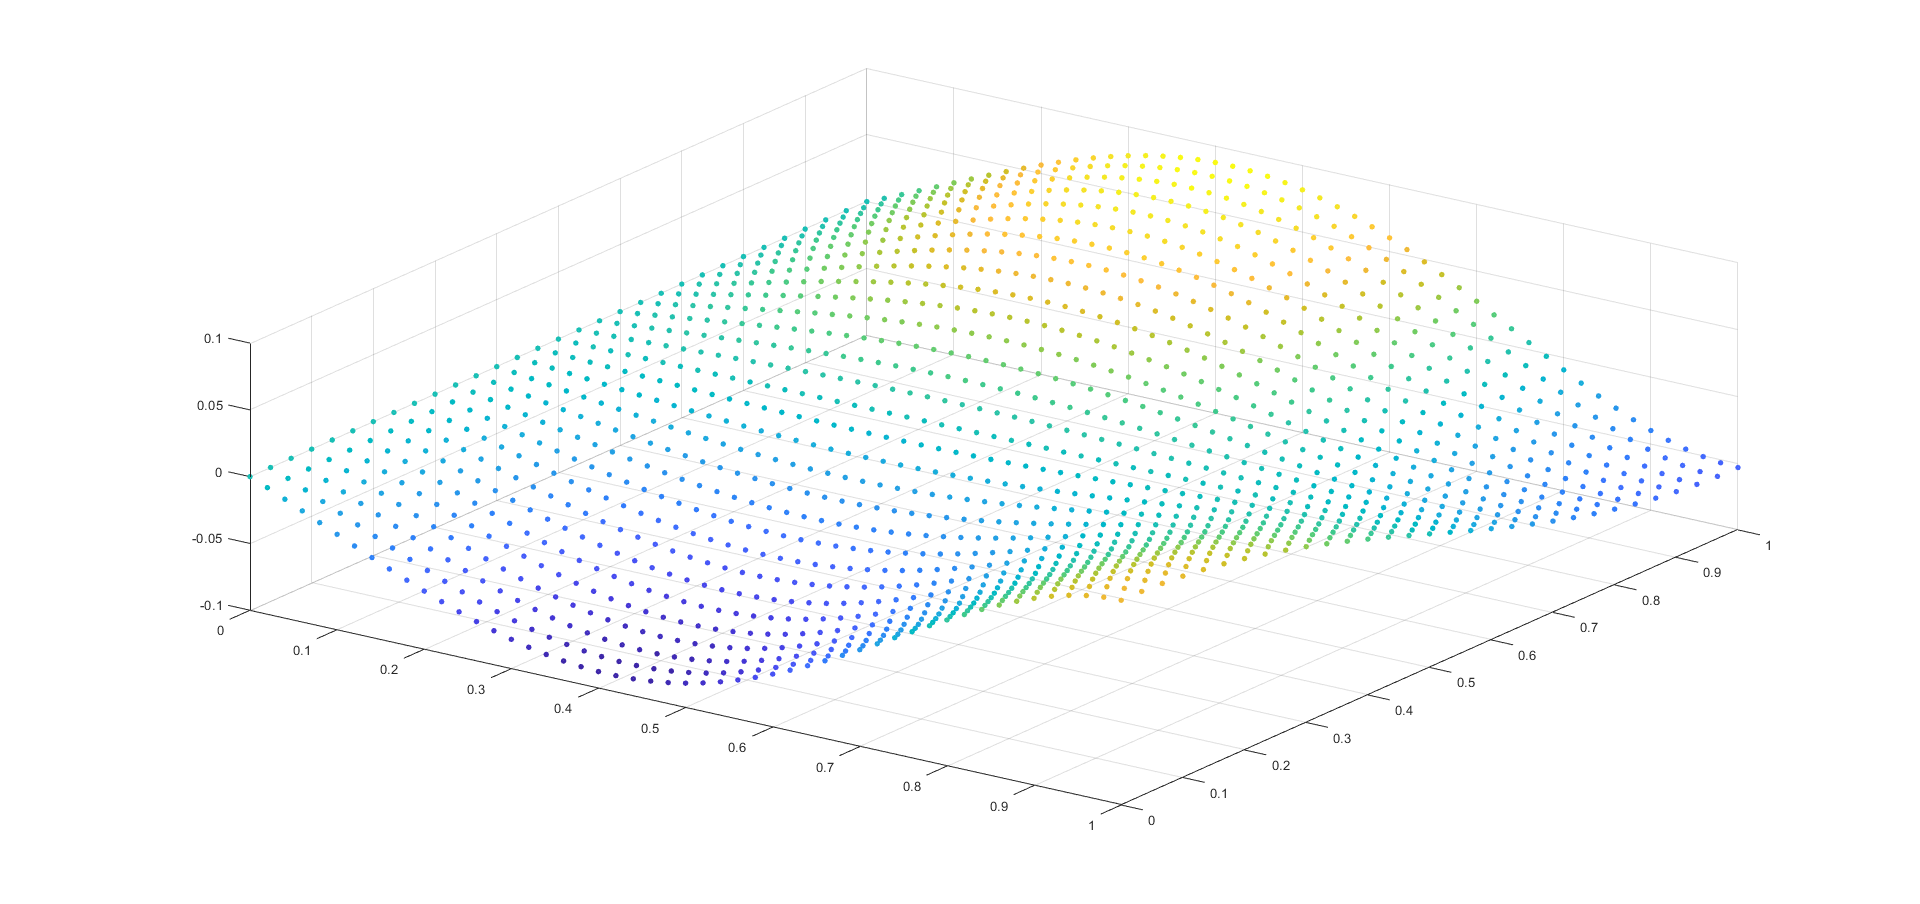
\includegraphics[width=1\linewidth]{Plate2.png}
				\subcaption{Plate - $\lambda_5 = 0.643$}
				\label{fig:minipage2}
			\end{minipage}
			\begin{minipage}[b]{0.8\linewidth}
				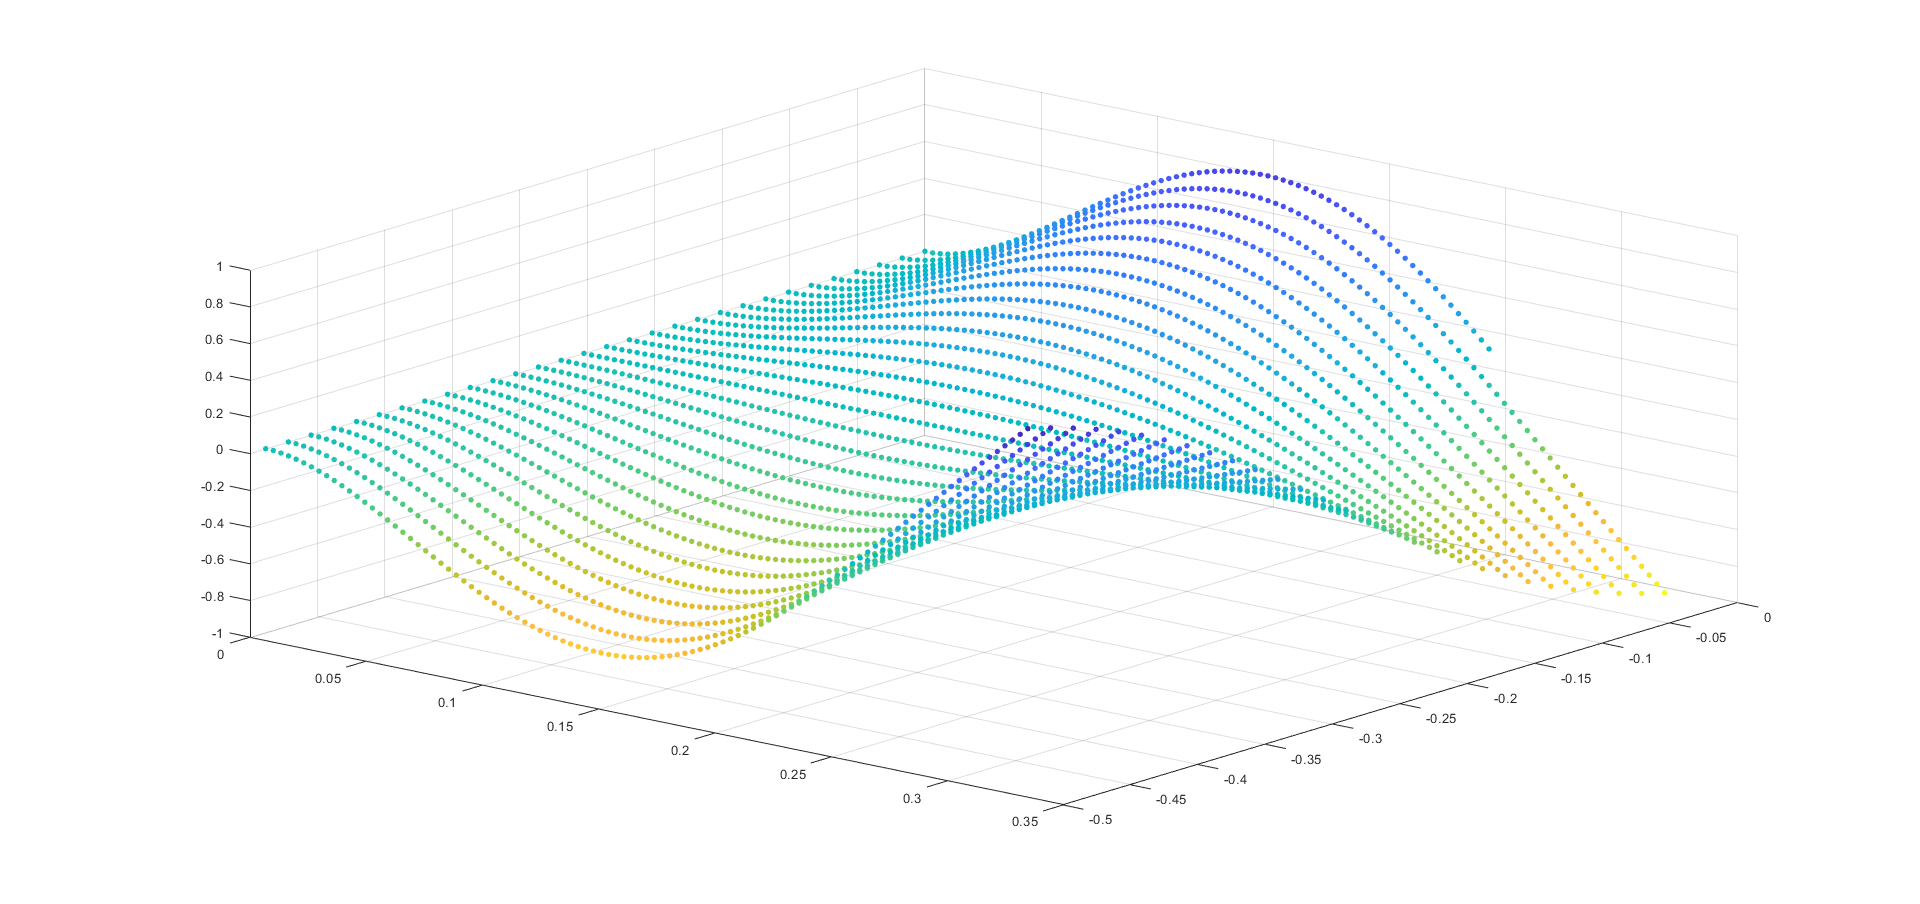
\includegraphics[width=1\linewidth]{3D2.png}
				\subcaption{3D Model - $\lambda_5 = 0.645$}
				\label{fig:minipage1}
			\end{minipage}
	}}
	\scalebox{.8}{
		\makebox[\textwidth][c]{
			\centering
			\begin{minipage}{.8\textwidth}
				\centering
				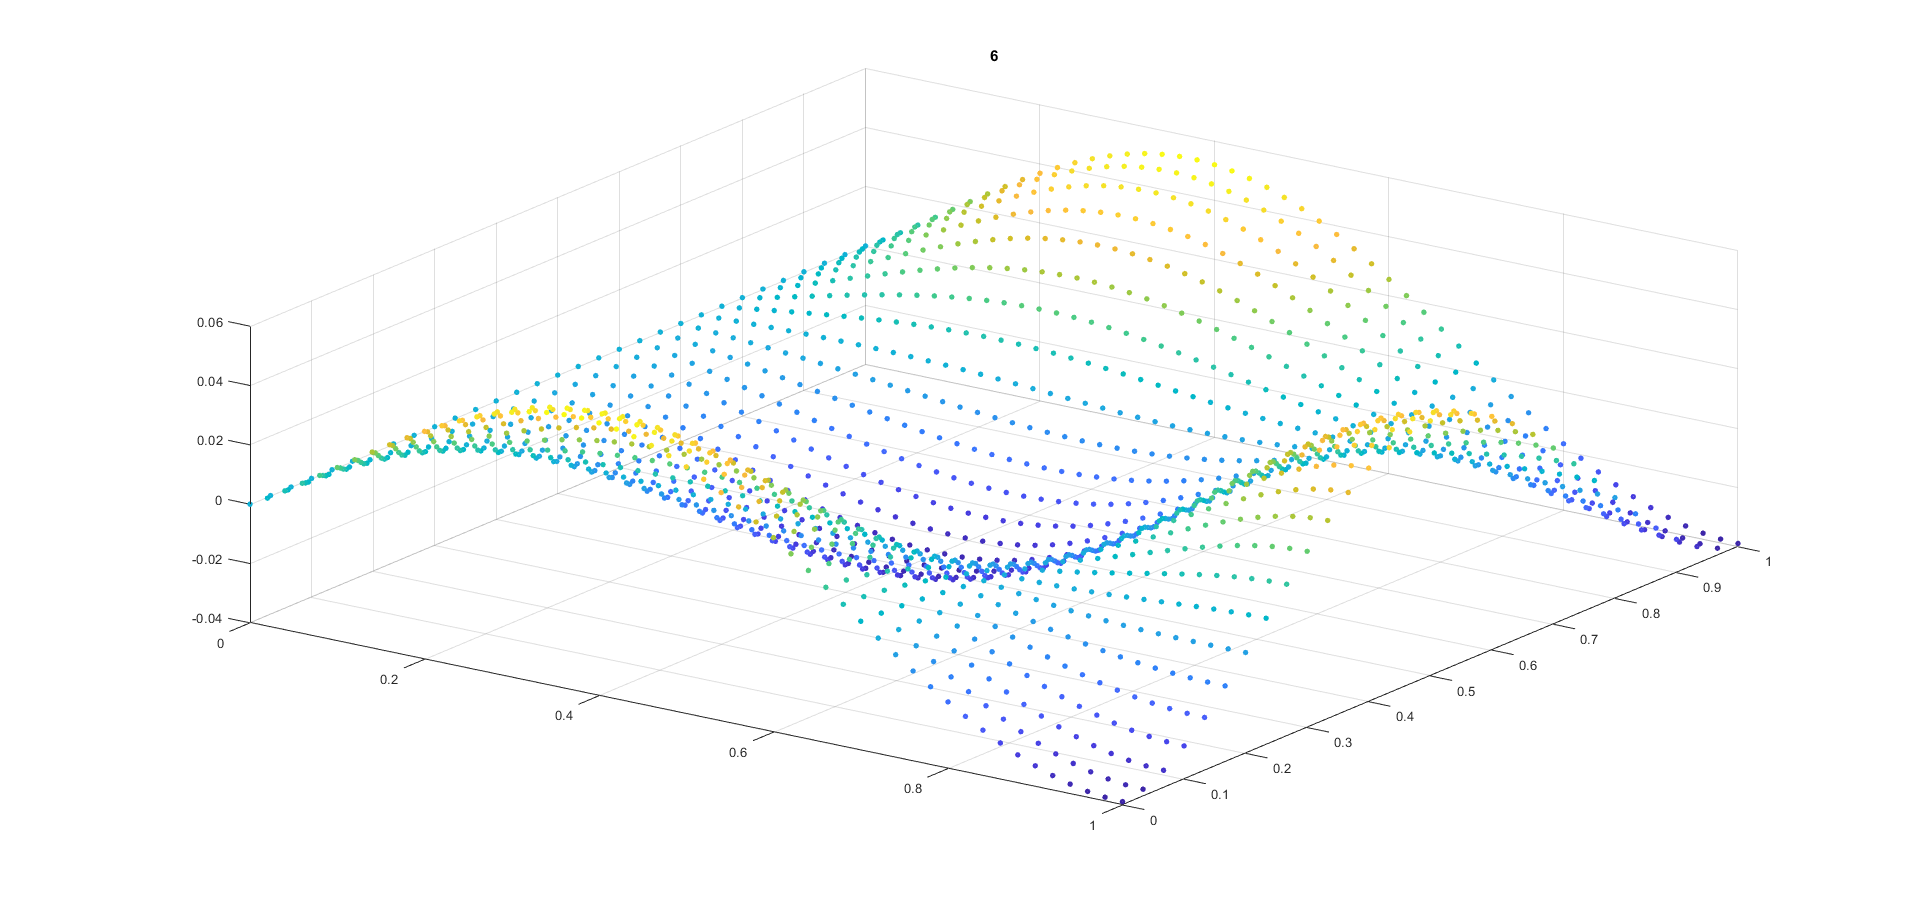
\includegraphics[width=1\linewidth]{Plate1.png}
				\subcaption{Plate - $\lambda_6 = 1.92$}
				\label{fig:minipage1}
			\end{minipage}
			\begin{minipage}{.8\textwidth}
				\centering
				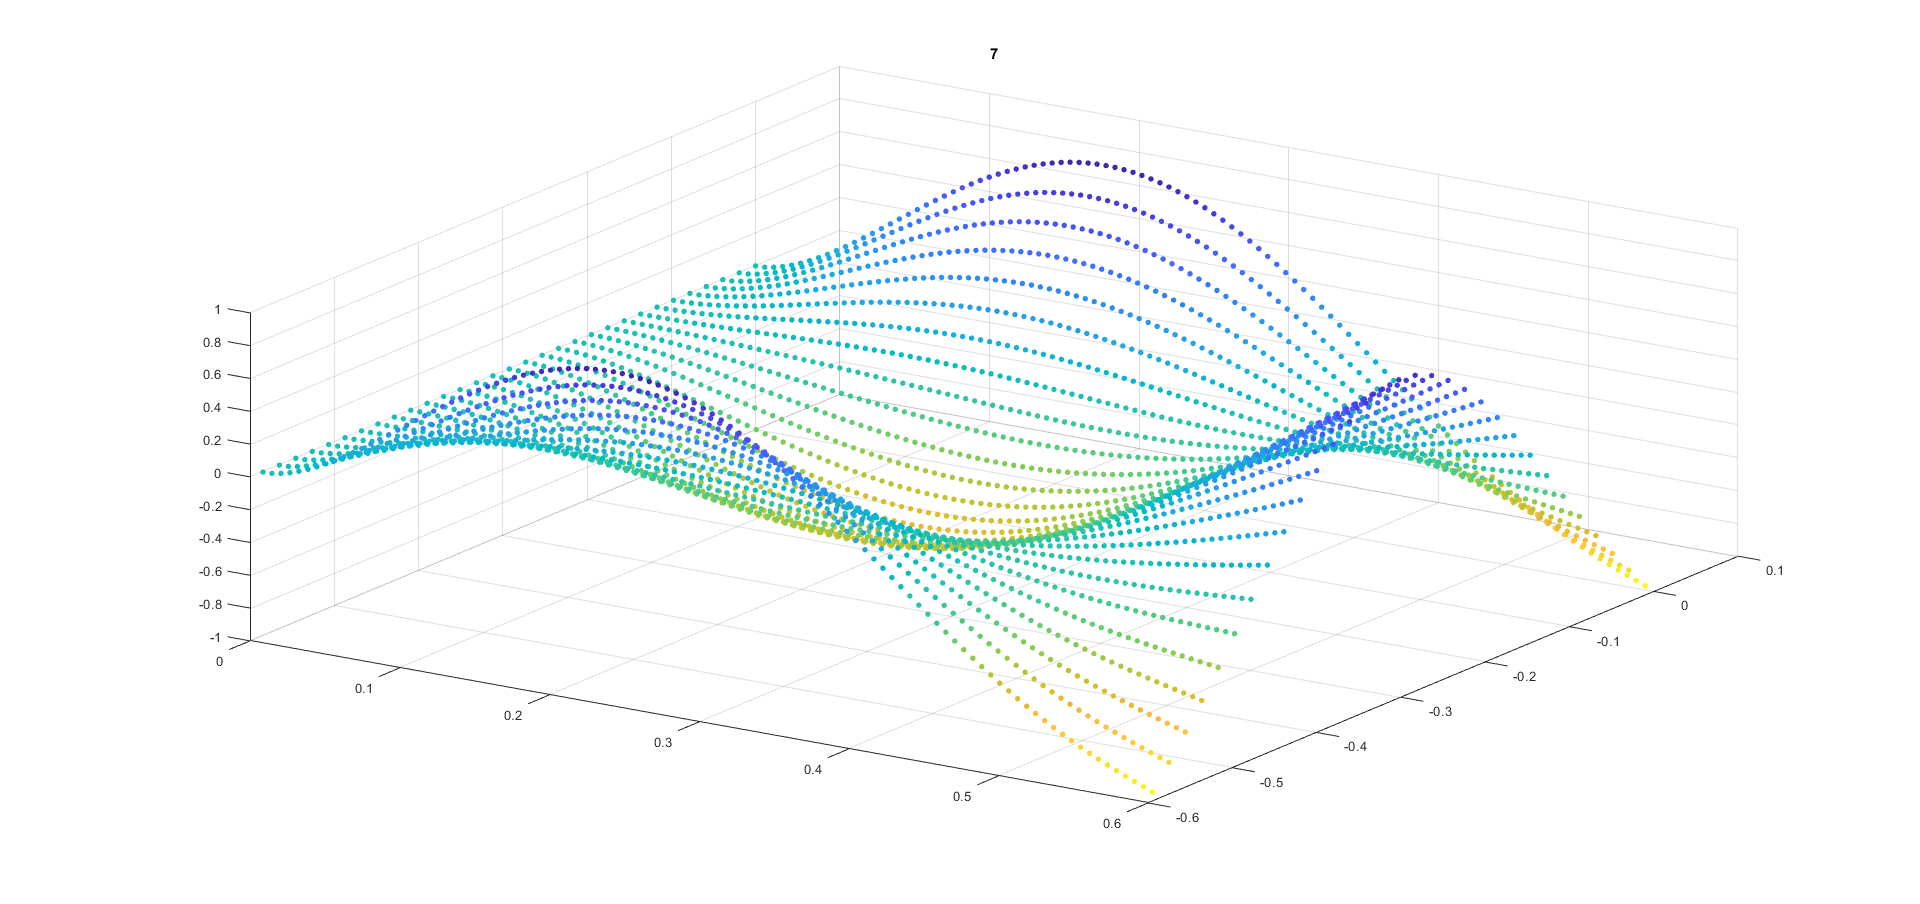
\includegraphics[width=1\linewidth]{3D1.png}
				\subcaption{3D Model - $\lambda_7 = 1.92$}
				\label{fig:minipage2}
			\end{minipage}
	}}
	\scalebox{.8}{
		\makebox[\textwidth][c]{
			\centering
			\begin{minipage}[b]{0.8\linewidth}
				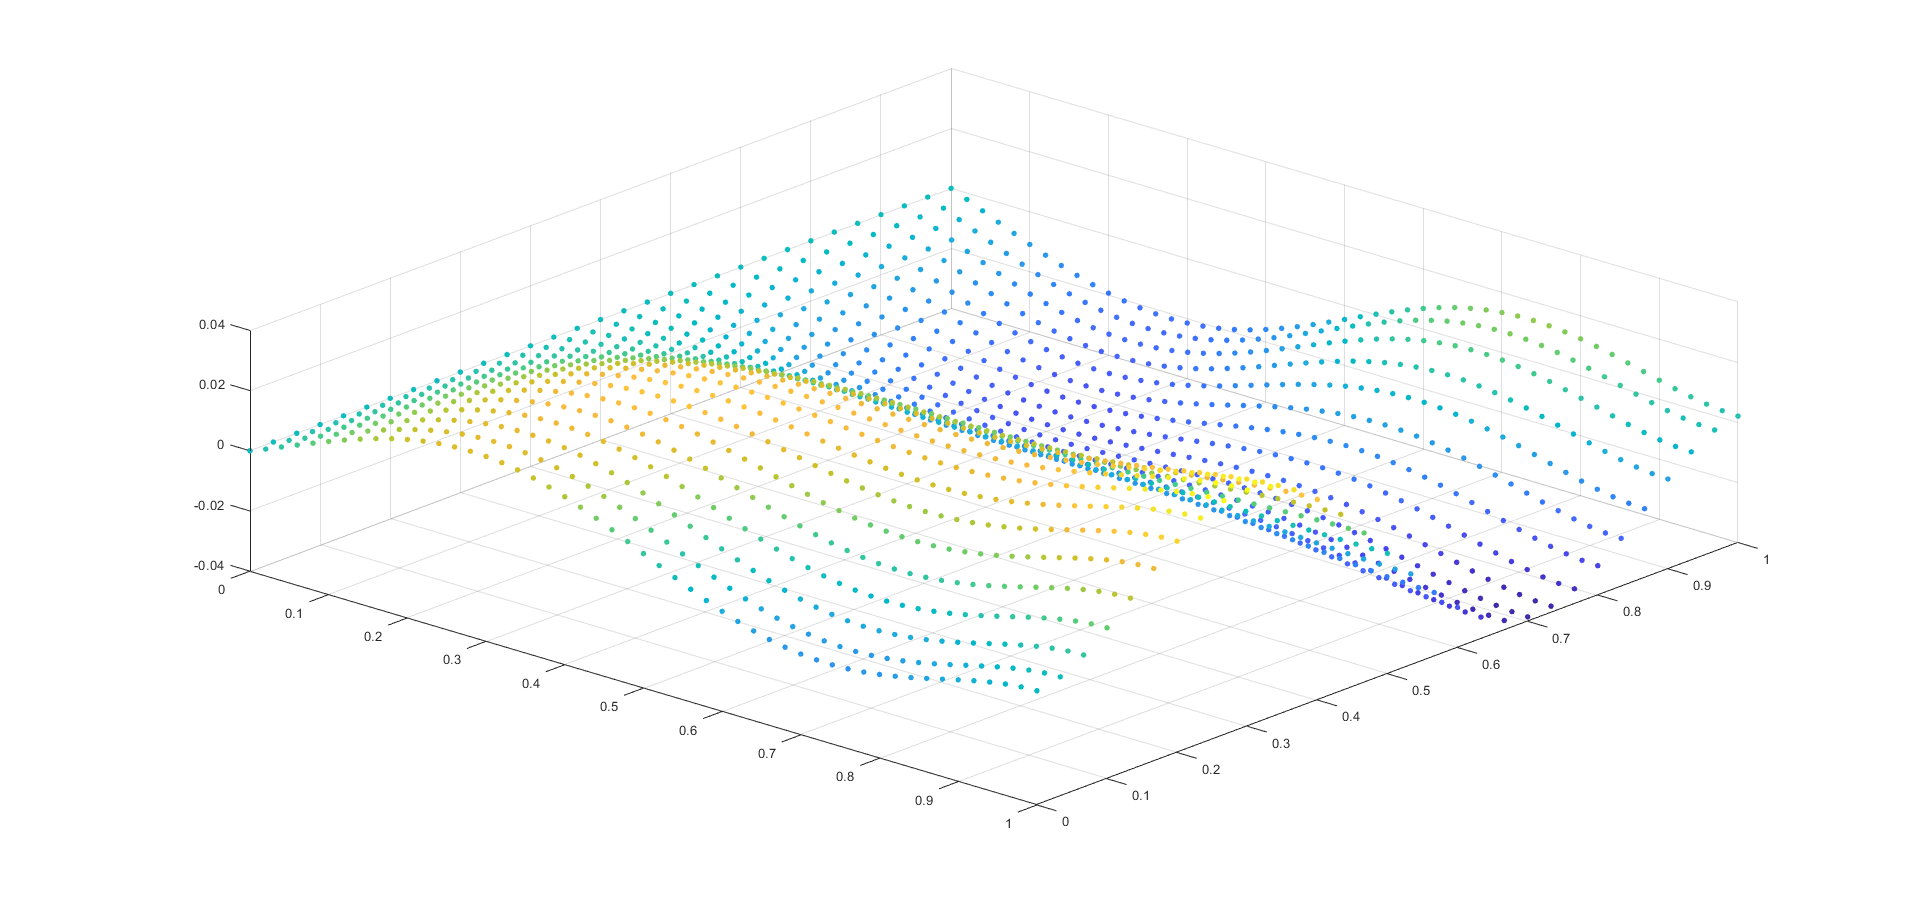
\includegraphics[width=1\linewidth]{Plate3.png}
				\subcaption{Plate - $\lambda_8 = 2.74$}
				\label{fig:minipage1}
			\end{minipage}
			\quad
			\begin{minipage}[b]{0.8\linewidth}
				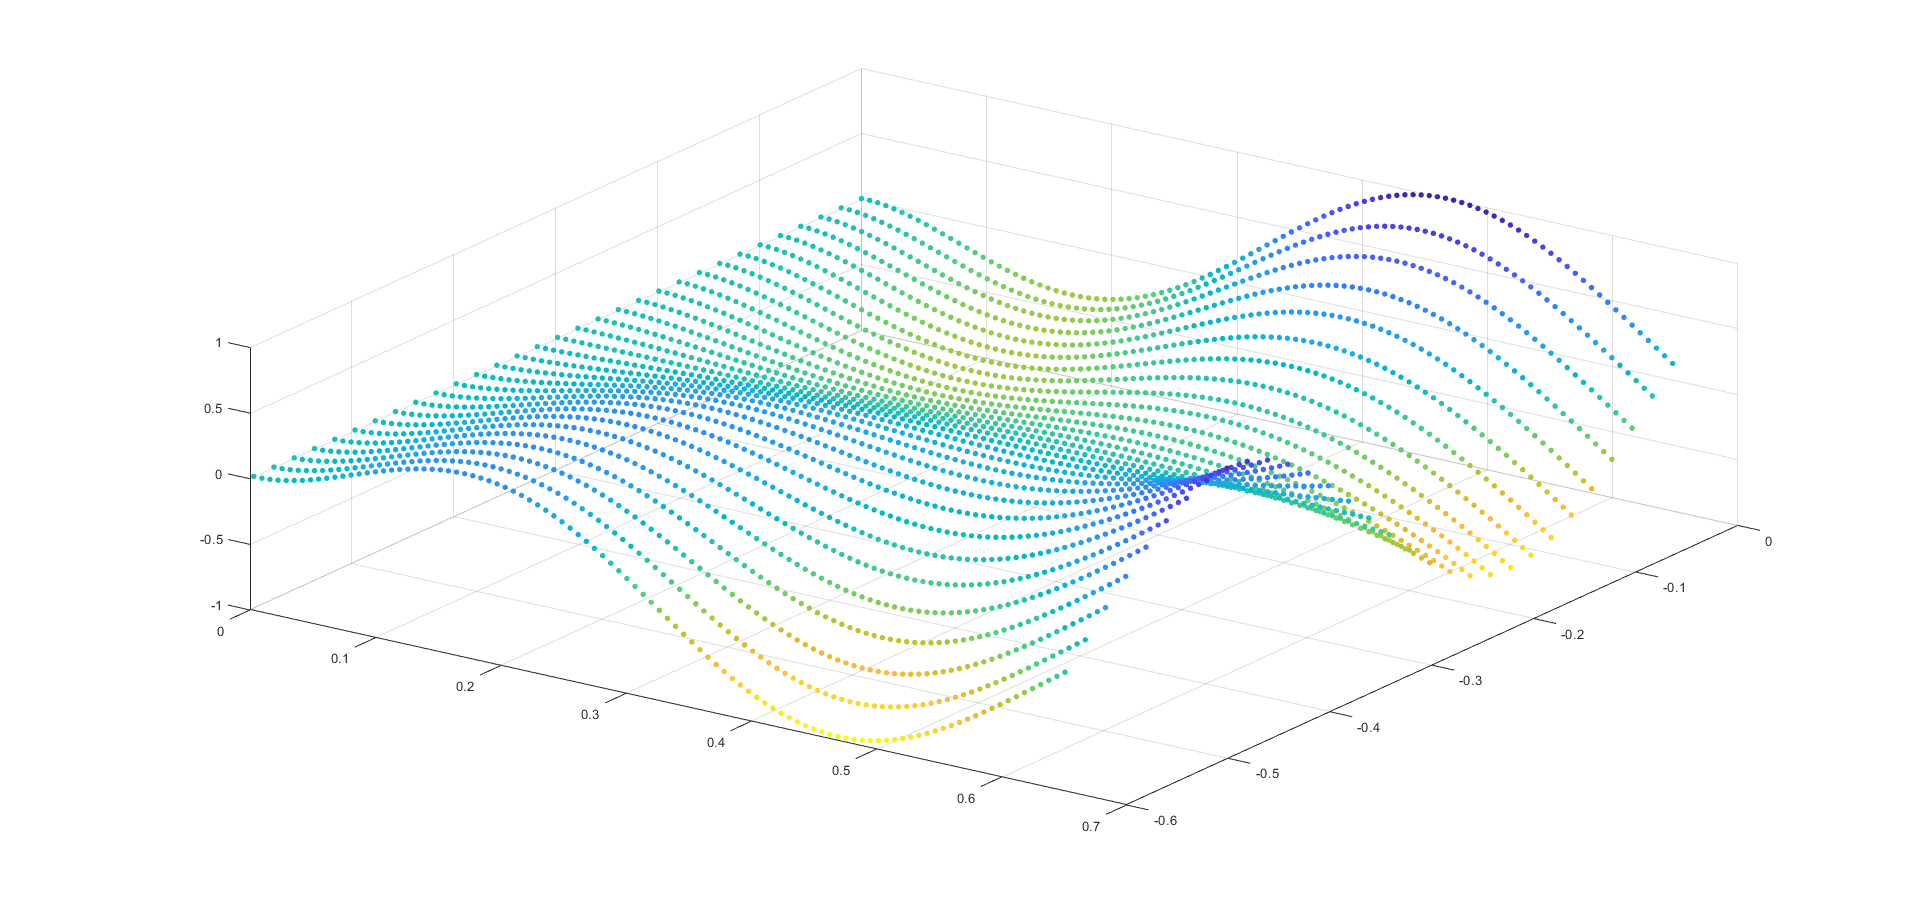
\includegraphics[width=1\linewidth]{3D3.png}
				\subcaption{3D Model - $\lambda_8 = 2.74$}
				\label{fig:minipage2}
			\end{minipage}
	}}
	\scalebox{.8}{
		\makebox[\textwidth][c]{
			\centering
			\begin{minipage}[b]{0.8\linewidth}
				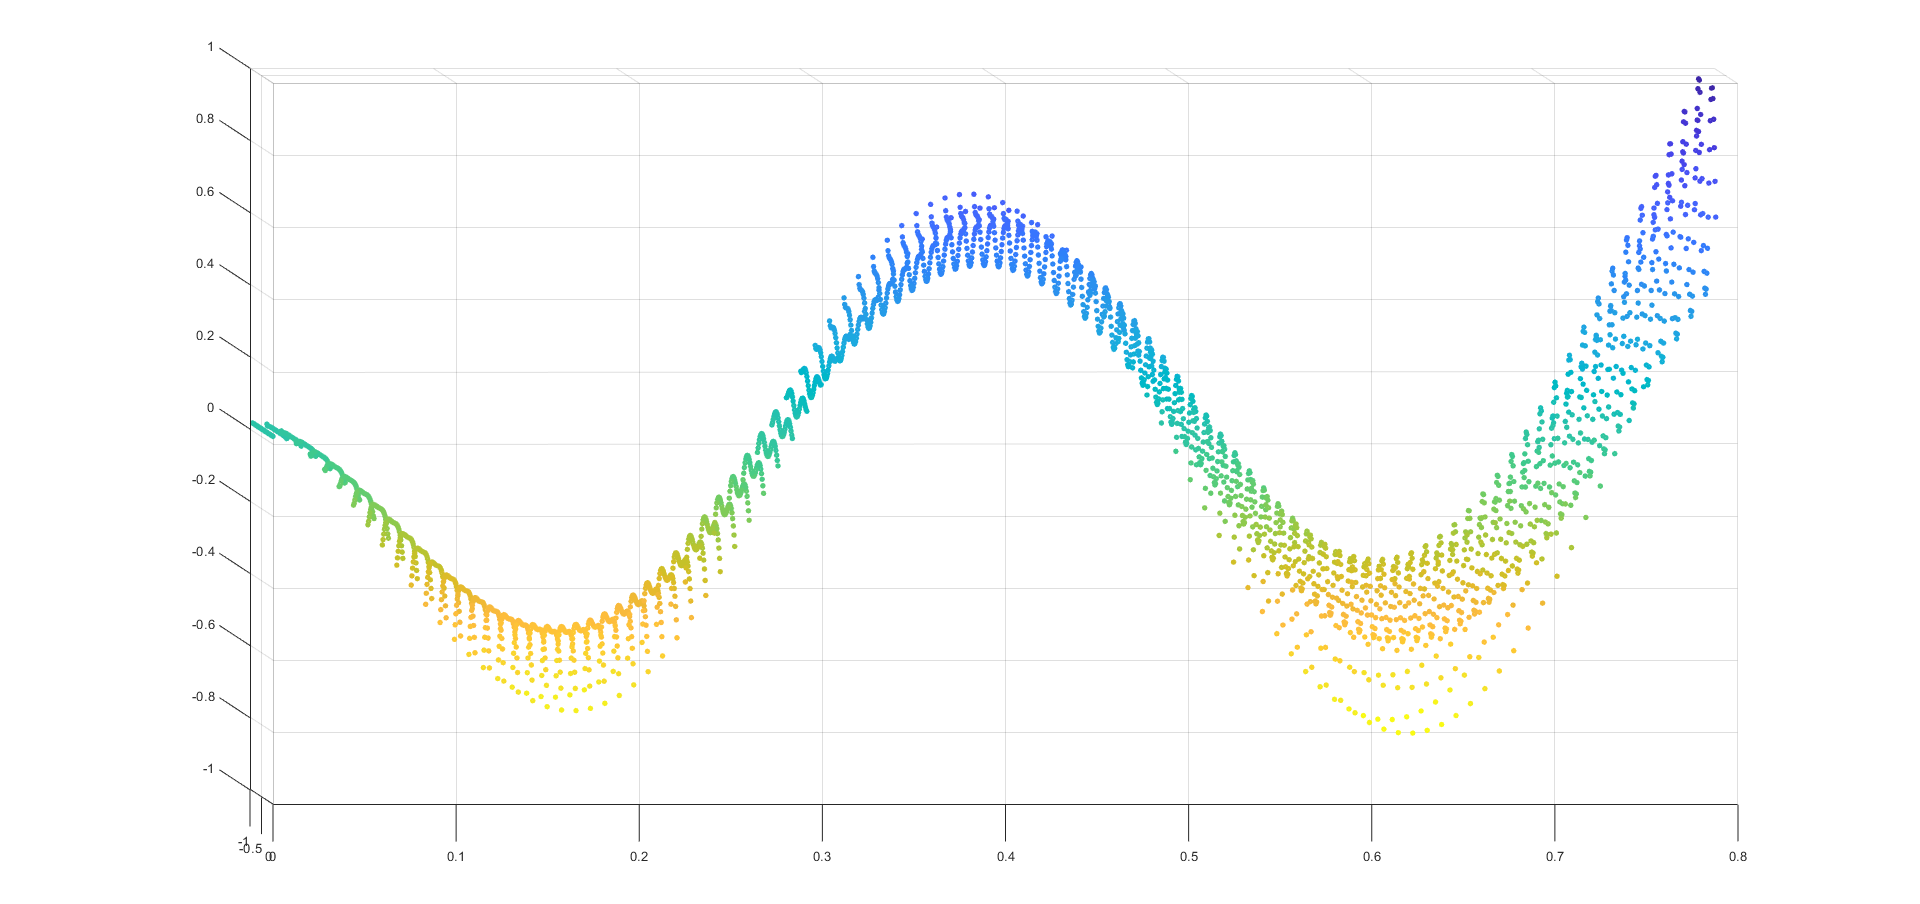
\includegraphics[width=1\linewidth]{Plate4.png}
				\subcaption{Plate - $\lambda_{12} = 8.96$ (Side view)}
				\label{fig:minipage2}
			\end{minipage}
			\quad
			\begin{minipage}[b]{0.8\linewidth}
				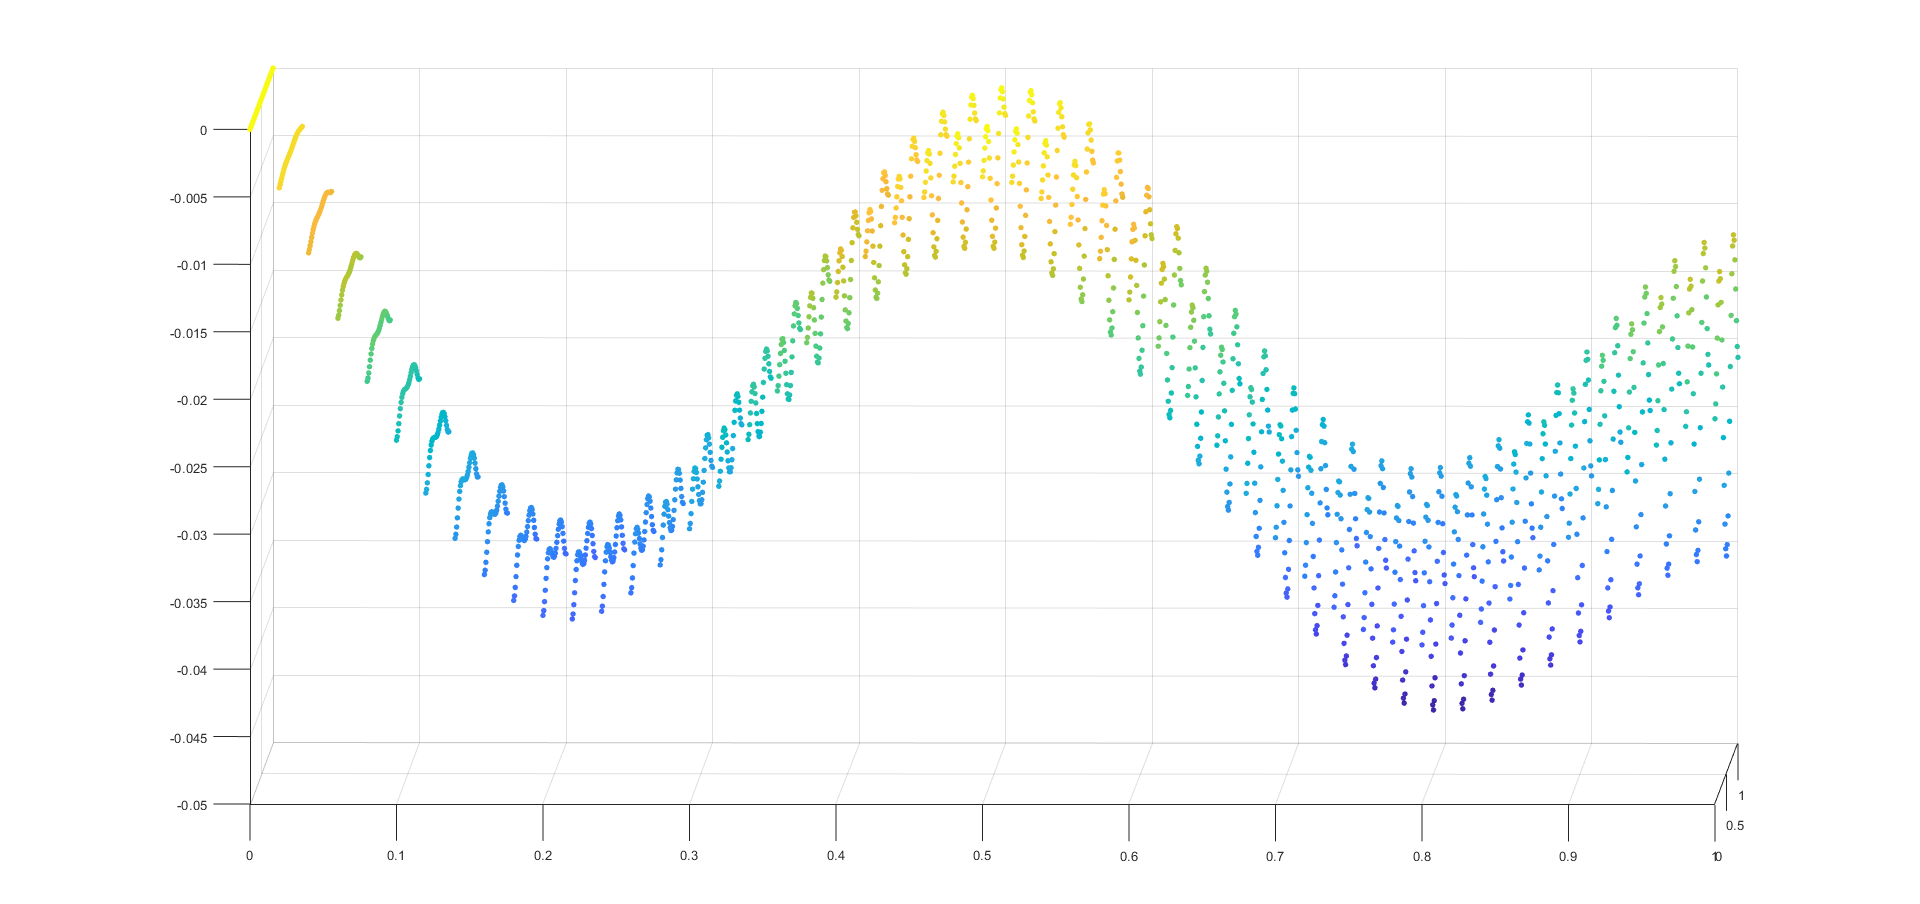
\includegraphics[width=1\linewidth]{3D4.png}
				\subcaption{3D Model - $\lambda_{14} = 9.01$ (Side view)}
				\label{fig:minipage2}
			\end{minipage}
			\caption{Comparison of Mode Shapes of the 3D model and the plate model. $b = 1/20$, $d = 1$.}
	}}
\end{figure}

\FloatBarrier


Let $b= 1$ and $\alpha= 4800$ so that $h= \frac{1}{2}$.\\

\begin{figure}[h!]
	\scalebox{.8}{
		\makebox[\textwidth][c]{
			\centering
			\begin{minipage}{.8\textwidth}
				\centering
				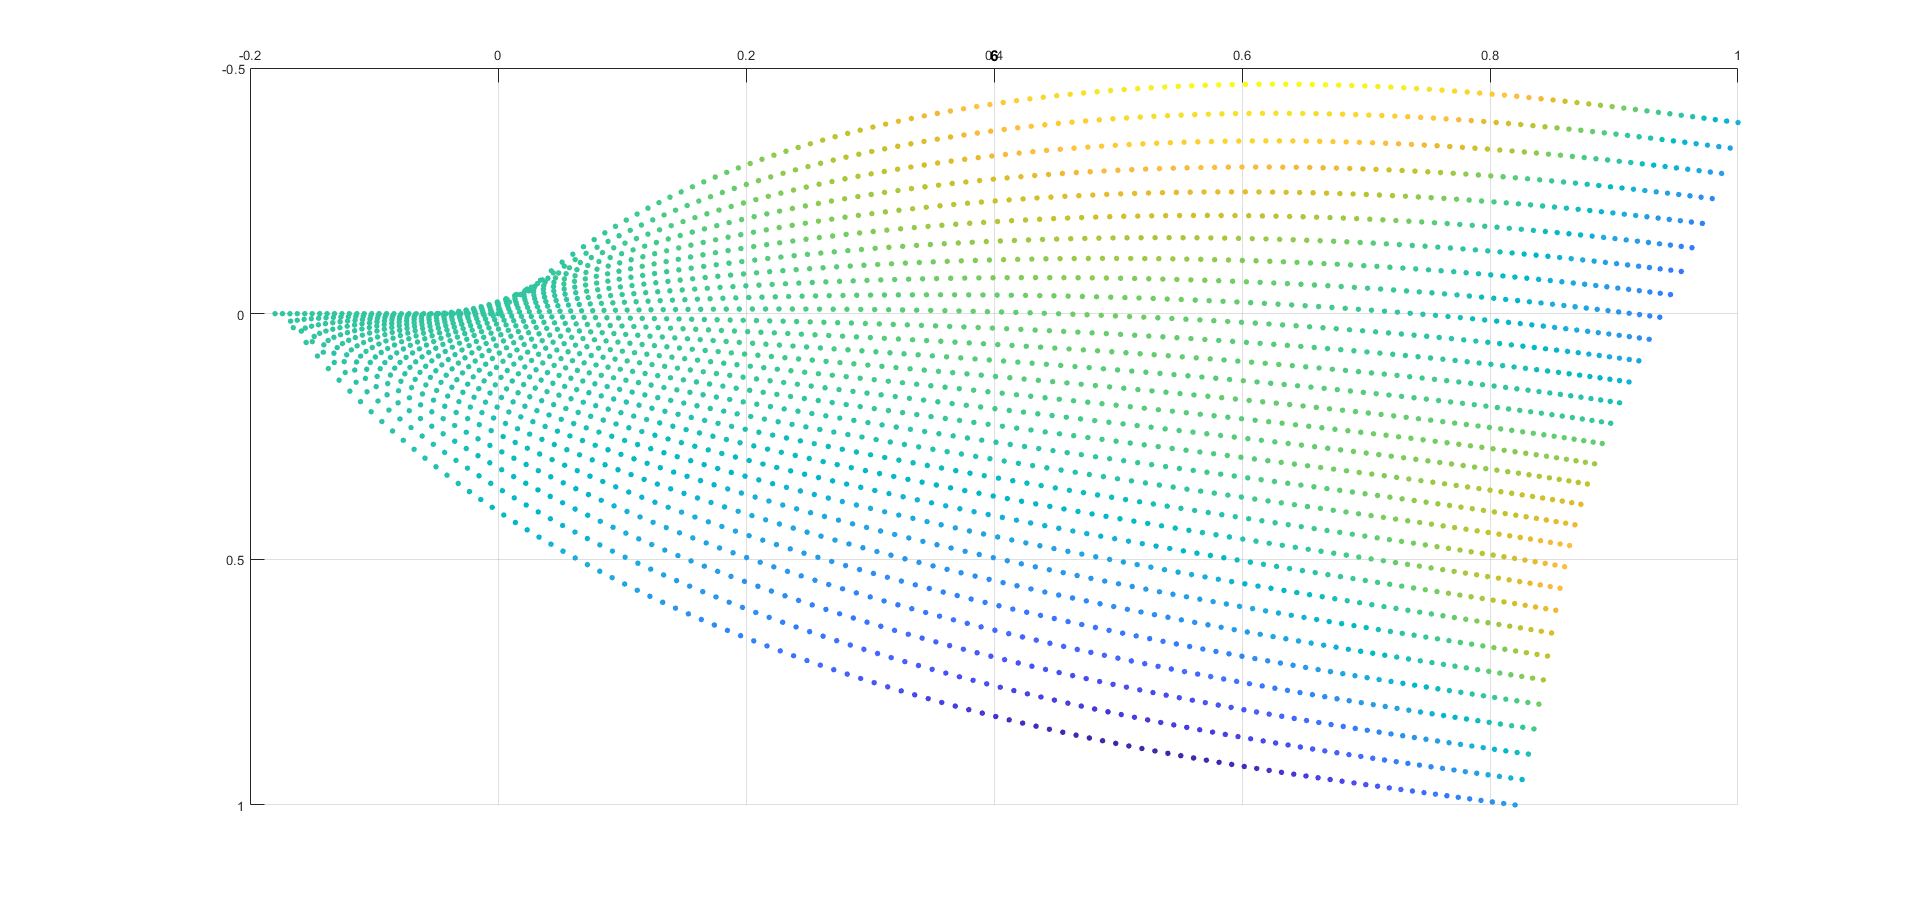
\includegraphics[width=1\linewidth]{3Dnp1.png}
				\subcaption{3D Model - $\lambda_{6} = 1.35$ (Top view)}
				\label{fig:minipage1}
			\end{minipage}
			\begin{minipage}{.8\textwidth}
				\centering
				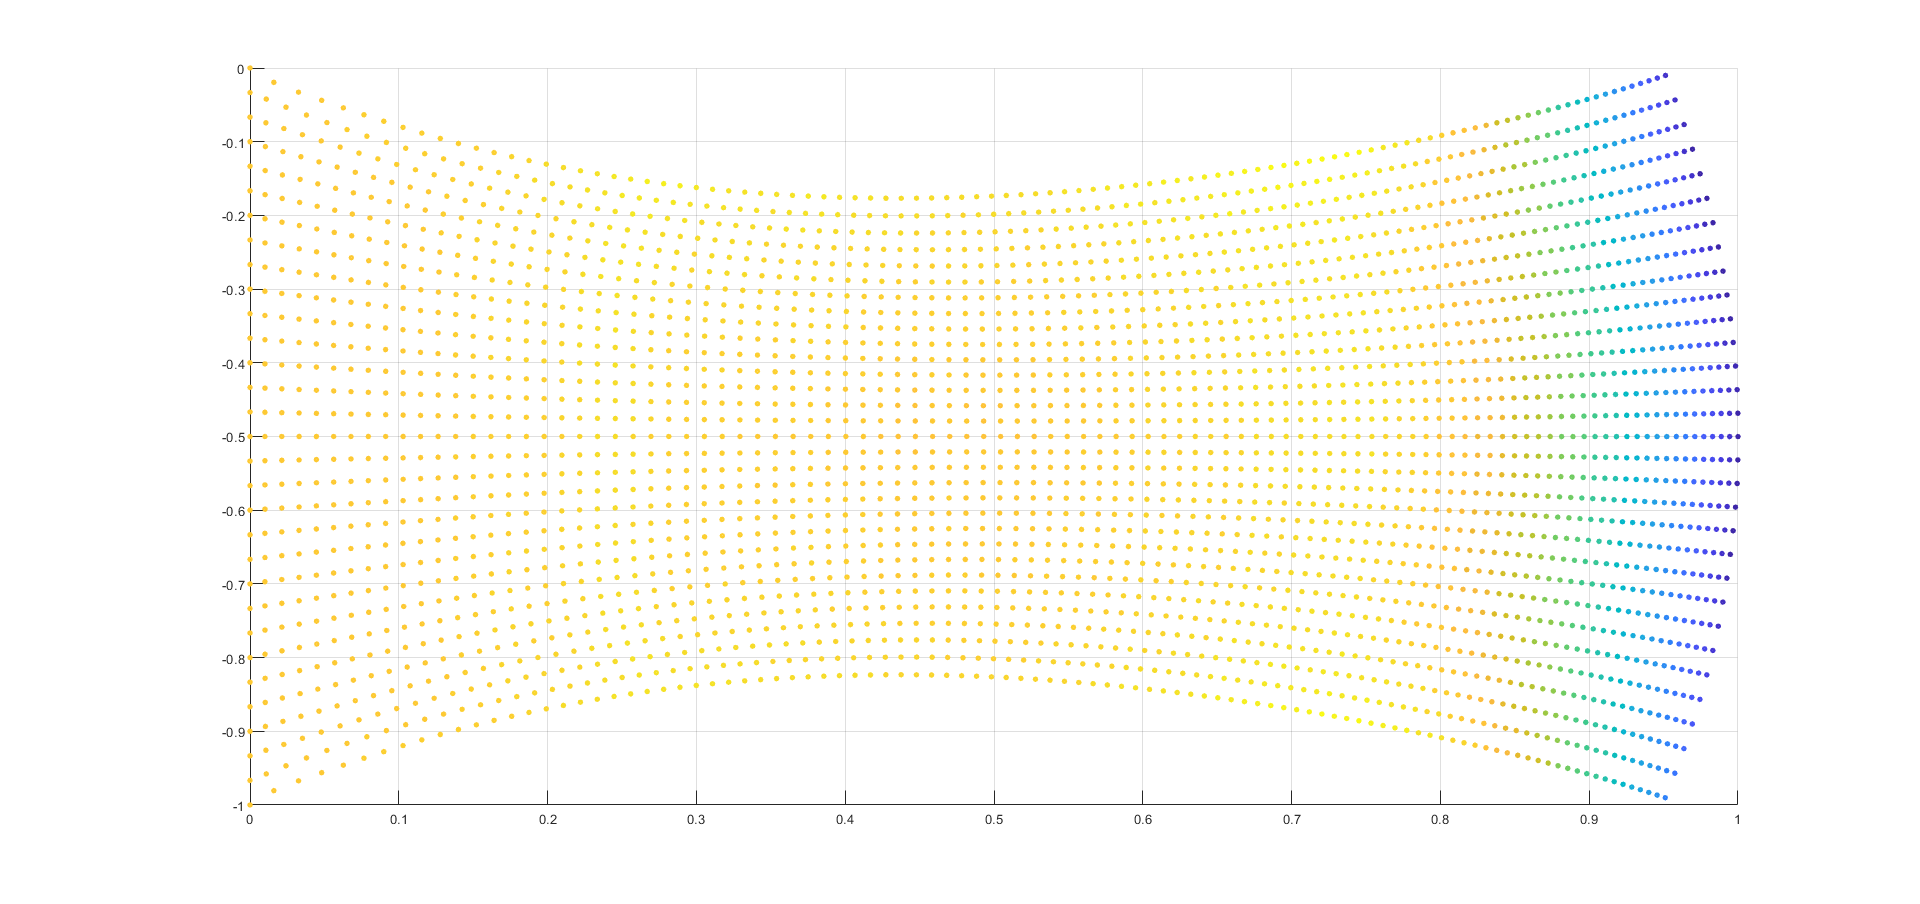
\includegraphics[width=1\linewidth]{3Dnp2.png}
				\subcaption{3D Model - $\lambda_{13} = 7.80$ (Top view)}
				\label{fig:minipage2}
			\end{minipage}
	}}
	\caption{Examples of non-plate mode shapes.}
\end{figure}

\subsection{Comparing the eigenvalues}
Tables \ref{tab:Table_plate_1} and \ref{tab:Table_plate_1} compare the eigenvalues of a cantilever Reissner-Mindlin plate model to the eigenvalues of a cantilever three-dimensional plate model. The different widths of plates considered are $b = 0.25$ and $b = 1$. These cases represent a slightly and very wide plate models. In each of the tables, the parameter $h$ representing the height is decreased.

\FloatBarrier
\begin{table}[htbp]
	\scalebox{.8}{
	\makebox[\textwidth]{
		\caption{Comparison of eigenvalues of the cantilever Reissner-Mindlin and three-dimensional plates.}
		\begin{tabular}{|cccc||cccc||cccc||cccc|}
			\hline
			\multicolumn{16}{|c|}{Comparison of Eigenvalues, $b = 0.25$} \\
			\hline\hline
			\multicolumn{4}{|c||}{$h = 1/5$}       & \multicolumn{4}{c||}{$h =1/10$}      & \multicolumn{4}{c||}{$h = 1/20$}      & \multicolumn{4}{c|}{$h = 1/30$} \\
			\hline
			{i} & {3D} & {j} & {Plate} & {i} & {3D} & {j} & {Plate} & {i} & {3D} & {j} & {Plate} & {i} & {3D} & {j} & {Plate} \\
			\hline
			1     & 0.12348 & 1     & {0.12249} & 1     & 0.032327 & 1     & 0.032184 & 1     & 0.008207 & 1     & 0.008186 & 1     & 0.003663 & 1     & 0.003656 \\
			2     & 0.18638 &       & -     & 2     & 0.18531 &       & {-} & 2     & 0.18476 &       & {-} & 2     & 0.14204 & 2     & 0.14173 \\
			3     & 2.4151 & 2     & {2.3954} & 3     & 1.161 & 2     & 1.1537 & 3     & 0.31436 & 2     & 0.31341 & 3     & 0.18456 &       & {-} \\
			4     & 3.5856 & 3     & {3.5368} & 4     & 1.3155 & 3     & 1.31  & 4     & 0.44696 & 3     & 0.44582 & 4     & 0.21514 & 3     & 0.21454 \\
			5     & 4.785 &       & -     & 5     & 4.7697 &       & {-} & 5     & 2.3862 & 4     & 2.3767 & 5     & 1.1001 & 4     & 1.0971 \\
			6     & 7.7889 &       & -     & 6     & 7.7674 & 4     & 7.9816 & 6     & 4.1984 & 5     & 4.1857 & 6     & 2.0374 & 5     & 2.0313 \\
			7     & 20.37 & 4     & {19.969} & 7     & 8.056 &       & {-} & 7     & 4.7615 &       & {-} & 7     & 4.1509 & 6     & 4.1367 \\
			8     & 21.722 & 5     & {21.537} & 8     & 12.034 & 5     & 11.972 & 8     & 7.7543 &       & {-} & 8     & 4.7585 &       & {-} \\
			9     & 25.181 &       & -     & 9     & 25.147 &       & {-} & 9     & 8.7609 & 6     & 8.7132 & 9     & 6.2078 & 7     & 6.1864 \\
			10    & 56.321 & 6     & {54.887} & 10    & 26.608 & 6     & 26.266 & 10    & 12.598 & 7     & 12.548 & 10    & 7.7495 &       & {-} \\
			11    & 60.267 & 7     & {59.71} & 11    & 34.438 & 7     & 34.197 & 11    & 22.619 & 8     & 22.456 & 11    & 11.064 & 8     & 11.015 \\
			12    & 65.513 &       & -     & 12    & 61.829 & 8     & 60.801 & 12    & 25.128 &       & {-} & 12    & 13.734 & 9     & 13.678 \\
			13    & 69.031 &       & -     & 13    & 65.518 &       & {-} & 13    & 27.297 & 9     & 27.155 & 13    & 23.854 & 10    & 23.724 \\
			14    & 114.09 & 8     & {110.7} & 14    & 69.133 & 9     & 69.548 & 14    & 47.123 & 10    & 46.695 & 14    & 25.121 &       & {-} \\
			15    & 117.88 & 9     & {116.66} & 15    & 70.211 &       & {-} & 15    & 50.515 & 11    & 50.174 & 15    & 26.054 & 11    & 25.927 \\
			16    & 127.05 &       & -     & 16    & 116.78 & 10    & 114.43 & 16    & 65.523 &       & {-} & 16    & 36.259 & 12    & 36.15 \\
			17    & 184.46 & 10    & {185.78} & 17    & 121.43 & 11    & 119.94 & 17    & 69.089 &       & {-} & 17    & 41.973 & 13    & 41.807 \\
			18    & 191.91 & 11    & {191.47} & 18    & 127.23 &       & {-} & 18    & 71.563 & 12    & 71.166 & 18    & 44.95 & 14    & 44.685 \\
			19    & 193.03 &       & -     & 19    & 178.27 & 12    & 175.79 & 19    & 81.444 & 13    & 80.894 & 19    & 45.798 & 15    & 45.507 \\
			20    & 193.71 &       & -     & 20    & 186.06 & 13    & 187.28 & 20    & 84.785 & 14    & 84.064 & 20    & 54.838 & 16    & 54.573 \\
			\hline
			\multicolumn{2}{|c}{Max RE:} & \multicolumn{2}{c||}{2.9764\%} & \multicolumn{2}{c}{Max RE:} & \multicolumn{2}{c||}{2.7585\%} & \multicolumn{2}{c}{Max RE:} & \multicolumn{2}{c||}{0.90845\%} & \multicolumn{2}{c}{Max RE:} & \multicolumn{2}{c|}{0.63525\%} \\
			\hline
		\end{tabular}%
		\label{tab:Table_plate_1}%
	}}
\end{table}%
\FloatBarrier

The results in Table \ref{tab:Table_plate_1} show that the cantilever Reissner-Mindlin plate model compare very well to the cantilever three-dimensional plate. For $h = 1/5$ the plate can be considered ``thick'', and the maximum relative error is less than $3\%$. This relative error decreases significantly as $h$ decreases.\\

As $b$ decreases, there are also more eigenvalues of the cantilever the Reissner-Mindlin plate relating to the first 20 eigenvalues of the cantilever three-dimensional plate. Table
\ref{tab:Table_plate_1_1} shows some more results for different values of $b$ without presenting the eigenvalues.


\FloatBarrier
\begin{table}[htbp]
	\centering
	\caption{Maximum relative error of the first 10 comparable eigenvalues with b = 0.25.}
	\begin{tabular}{|c|c|c|c|c|c|}
		\hline
		\multicolumn{6}{|c|}{Max Relative Error } \\ 
		\hline 
		\hline
		b = 1/2 & b = 1/5 & b = 1/10 & b = 1/20 & b = 1/30 & b = 1/50\\ \hline
		3.4514\% & 2.9764 \% & 2.7585 \% & 0.90845 \% & 0.63525 \% & 0.50397 \% \\ \hline
	\end{tabular}%
	\label{tab:Table_plate_1_1}%
\end{table}%

\FloatBarrier
\begin{table}[htbp]
	\scalebox{.8}{
	\makebox[\textwidth]{
		\caption{Comparison of eigenvalues of the cantilever Reissner-Mindlin and three-dimensional plates.}
		\begin{tabular}{|cccc||cccc||cccc||cccc|}
			\hline
			\multicolumn{16}{|c|}{Comparison of Eigenvalues, $b = 1$} \\
			\hline\hline
			\multicolumn{4}{|c||}{$h = 1/5$}       & \multicolumn{4}{c||}{$h =1/10$}      & \multicolumn{4}{c||}{$h = 1/20$}      & \multicolumn{4}{c|}{$h = 1/30$} \\
			\hline
			{i} & {3D} & {j} & {Plate} & {i} & {3D} & {j} & {Plate} & {i} & {3D} & {j} & {Plate} & {i} & {3D} & {j} & {Plate} \\
			\hline
			1     & 0.12869 & 1     & {0.12743} & 1     & 0.033784 & 1     & 0.033626 & 1     & 0.008565 & 1     & 0.008543 & 1     & 0.003817 & 1     & {0.00381} \\
			2     & 0.62189 & 2     & {0.61703} & 2     & 0.18635 & 2     & 0.18562 & 2     & 0.049829 & 2     & 0.04957 & 2     & 0.022511 & 2     & {0.022405} \\
			3     & 1.3638 &       & -     & 3     & 1.1603 & 3     & 1.153 & 3     & 0.31428 & 3     & 0.31315 & 3     & 0.14192 & 3     & {0.14156} \\
			4     & 3.5808 & 3     & {3.5289} & 4     & 1.3579 &       & {-} & 4     & 0.50842 & 4     & 0.50676 & 4     & 0.23035 & 4     & {0.22969} \\
			5     & 5.8165 & 4     & {5.7694} & 5     & 1.864 & 4     & 1.8577 & 5     & 0.64595 & 5     & 0.64297 & 5     & 0.29502 & 5     & {0.29394} \\
			6     & 6.6048 & 5     & {6.5216} & 6     & 2.2928 & 5     & 2.2792 & 6     & 1.3555 &       & {-} & 6     & 0.8928 & 6     & {0.88735} \\
			7     & 7.8455 &       & -     & 7     & 6.4973 & 6     & 6.4546 & 7     & 1.9293 & 6     & 1.9157 & 7     & 1.156 & 7     & {1.1527} \\
			8     & 9.8027 &       & -     & 8     & 7.8167 &       & {-} & 8     & 2.5089 & 7     & 2.4975 & 8     & 1.265 & 8     & {1.261} \\
			9     & 17.03 & 6     & {16.802} & 9     & 8.4533 & 7     & 8.3671 & 9     & 2.7486 & 8     & 2.7369 & 9     & 1.3543 &       & - \\
			10    & 21.225 & 7     & {20.743} & 10    & 9.3453 & 8     & 9.2873 & 10    & 3.3087 & 9     & 3.2903 & 10    & 1.5352 & 9     & {1.529} \\
			11    & 23.935 & 8     & {23.552} & 11    & 9.8009 &       & {-} & 11    & 5.5365 & 10    & 5.4914 & 11    & 2.598 & 10    & {2.5803} \\
			12    & 24.694 &       & -     & 12    & 10.925 & 9     & 10.827 & 12    & 5.9696 & 11    & 5.9246 & 12    & 2.8161 & 11    & {2.7997} \\
			13    & 27.187 & 9     & {26.69} & 13    & 17.599 & 10    & 17.447 & 13    & 7.8024 &       & {-} & 13    & 4.2654 & 12    & {4.2474} \\
			14    & 28.844 &       & -     & 14    & 18.596 & 11    & 18.407 & 14    & 9.0173 & 12    & 8.9573 & 14    & 4.6674 & 13    & {4.6415} \\
			15    & 32.373 &       & -     & 15    & 24.729 &       & {-} & 15    & 9.8006 & 13    & 9.838 & 15    & 4.9397 & 14    & {4.9143} \\
			16    & 41.288 & 10    & {40.519} & 16    & 27.4  & 12    & 27.021 & 16    & 9.9172 &       & {-} & 16    & 5.7243 & 15    & {5.6803} \\
			17    & 42.082 & 11    & {41.246} & 17    & 28.81 &       & {-} & 17    & 10.365 & 13    & 10.286 & 17    & 6.6585 & 16    & {6.6025} \\
			18    & 51.427 &       & -     & 18    & 30.737 & 13    & 30.413 & 18    & 11.934 & 14    & 11.817 & 18    & 7.2935 & 17    & {7.2474} \\
			19    & 56.963 & 12    & {56.1} & 19    & 30.83 & 14    & 30.413 & 19    & 13.915 & 15    & 13.767 & 19    & 7.7966 &       & - \\
			20    & 57.741 &       & -     & 20    & 32.414 &       &       & 20    & 15.109 & 16    & 14.974 & 20    & 9.7996 &       & - \\
			\hline
			\multicolumn{2}{|c}{Max RE:} & \multicolumn{2}{c||}{2.2695\%} & \multicolumn{2}{c}{Max RE:} & \multicolumn{2}{c||}{1.3816\%} & \multicolumn{2}{c}{Max RE:} & \multicolumn{2}{c||}{1.0657\%} & \multicolumn{2}{c}{Max RE:} & \multicolumn{2}{c|}{0.84102\%} \\
			\hline
		\end{tabular}%
		\label{tab:Table_plate_2}%
	}}
\end{table}%
\FloatBarrier

Similarly, Table \ref{tab:Table_plate_2} also show that a cantilever Reissner-Mindlin plate compares very well to a cantilever three-dimensional plate for $b=1$ which can be considered a wide plate.\\

Table \ref{tab:Table_plate_2_2} presents some more results without showing all the eigenvalues.


\FloatBarrier
\begin{table}[htbp]
	\centering
	\caption{Maximum relative error of the first 10 comparable eigenvalues with d=1.}
	\begin{tabular}{|c|c|c|c|c|c|}
		\hline
		\multicolumn{6}{|c|}{Max Relative Error } \\ 
		\hline 
		\hline
		b = 1/2 & b = 1/5 & b = 1/10 & b = 1/20 & b = 1/30 & b = 1/50\\ \hline
		3.9342\% & 2.2695 \% & 1.3816 \% & 1.0657 \% & 0.84101 \% & 0.38181 \% \\ \hline
	\end{tabular}%
	\label{tab:addlabel}%
\end{table}%


\FloatBarrier
\begin{table}[htbp]
	\scalebox{.8}{
	\makebox[\textwidth]{
		\caption{Comparison of eigenvalues of the cantilever Reissner-Mindlin and three-dimensional plates.}
		\begin{tabular}{|cccc||cccc||cccc||cccc|}
			\hline
			\multicolumn{16}{|c|}{Comparison of Eigenvalues, $b = 1.75$} \\
			\hline\hline
			\multicolumn{4}{|c||}{$h = 1/5$}       & \multicolumn{4}{c||}{$h =1/10$}      & \multicolumn{4}{c||}{$h = 1/20$}      & \multicolumn{4}{c|}{$h = 1/30$} \\
			\hline
			{i} & {3D} & {j} & {Plate} & {i} & {3D} & {j} & {Plate} & {i} & {3D} & {j} & {Plate} & {i} & {3D} & {j} & {Plate} \\
			\hline
			1 & 0.13062 & 1 & 0.12939 & 1 & 0.03425 & 1 & 0.03408 & 1 & 0.00867 & 1 & 0.00865 & 1 & 0.00386 & 1 & 0.00385 \\
			2 & 0.32016 & 2 & 0.31779 & 2 & 0.08987 & 2 & 0.08951 & 2 & 0.02339 & 2 & 0.02332 & 2 & 0.01051 & 2 & 0.01048 \\
			3 & 1.24962 & 3 & 1.24217 & 3 & 0.36964 & 3 & 0.36841 & 3 & 0.09807 & 3 & 0.09774 & 3 & 0.04424 & 3 & 0.04407 \\
			4 & 1.98080 & 4 & - & 4 & 1.22744 & 4 & 1.21878 & 4 & 0.33233 & 4 & 0.33118 & 4 & 0.15003 & 4 & 0.14964 \\
			5 & 3.76748 & 5 & 3.70863 & 5 & 1.35201 & 5 & 1.34648 & 5 & 0.36764 & 5 & 0.36652 & 5 & 0.16657 & 5 & 0.16605 \\
			6 & 4.20207 & 6 & 4.16307 & 6 & 1.69937 & 6 & 1.68940 & 6 & 0.46470 & 6 & 0.46320 & 6 & 0.21059 & 6 & 0.21002 \\
			7 & 5.20220 & 7 & 5.13810 & 7 & 1.97634 & 7 & - & 7 & 0.79935 & 7 & 0.79606 & 7 & 0.36560 & 7 & 0.36423 \\
			8 & 7.66031 & 8 & - & 8 & 7.93990 & 8 & - & 8 & 2.82592 & 8 & 2.80764 & 8 & 1.24449 & 8 & 1.24107 \\
			9 & 8.04452 & 9 & - & 9 & 4.45065 & 9 & 4.42937 & 9 & 1.57085 & 9 & 1.56301 & 9 & 0.72384 & 9 & 0.72032 \\
			10 & 9.07913 & 10 & - & 10 & 5.39232 & 10 & 5.35391 & 10 & 1.97389 & 10 & - & 10 & 1.15848 & 10 & 1.15447 \\
			11 & 10.13456 & 11 & - & 11 & 7.63711 & 11 & - & 11 & 2.51366 & 11 & 2.50221 & 11 & 1.13338 & 11 & 1.13071 \\
			12 & 11.18698 & 12 & - & 12 & 9.38184 & 12 & - & 12 & 3.16638 & 12 & - & 12 & 1.47191 & 12 & - \\
			% More rows can be added as per your data...
			\hline
			\multicolumn{2}{|c}{Max RE:} & \multicolumn{2}{c||}{-} & \multicolumn{2}{c}{Max RE:} & \multicolumn{2}{c||}{-} & \multicolumn{2}{c}{Max RE:} & \multicolumn{2}{c||}{-} & \multicolumn{2}{c}{Max RE:} & \multicolumn{2}{c|}{-} \\
			\hline
		\end{tabular}%
		\label{tab:Table_plate_full}%
	}}
\end{table}%
\FloatBarrier



\end{document}
